\chapter{Ergebnisse und Auswertung}
\label{ergebnisse}

% TODO: entweder Bezug auf die Fragen aus Kapitel 5 nehmen oder se ganz weg lassen

\section{Tempofehler}
{
	\subsection{Ergebnisse}
	{
		\begin{figure}[h]
			\hspace{-2.8cm}
			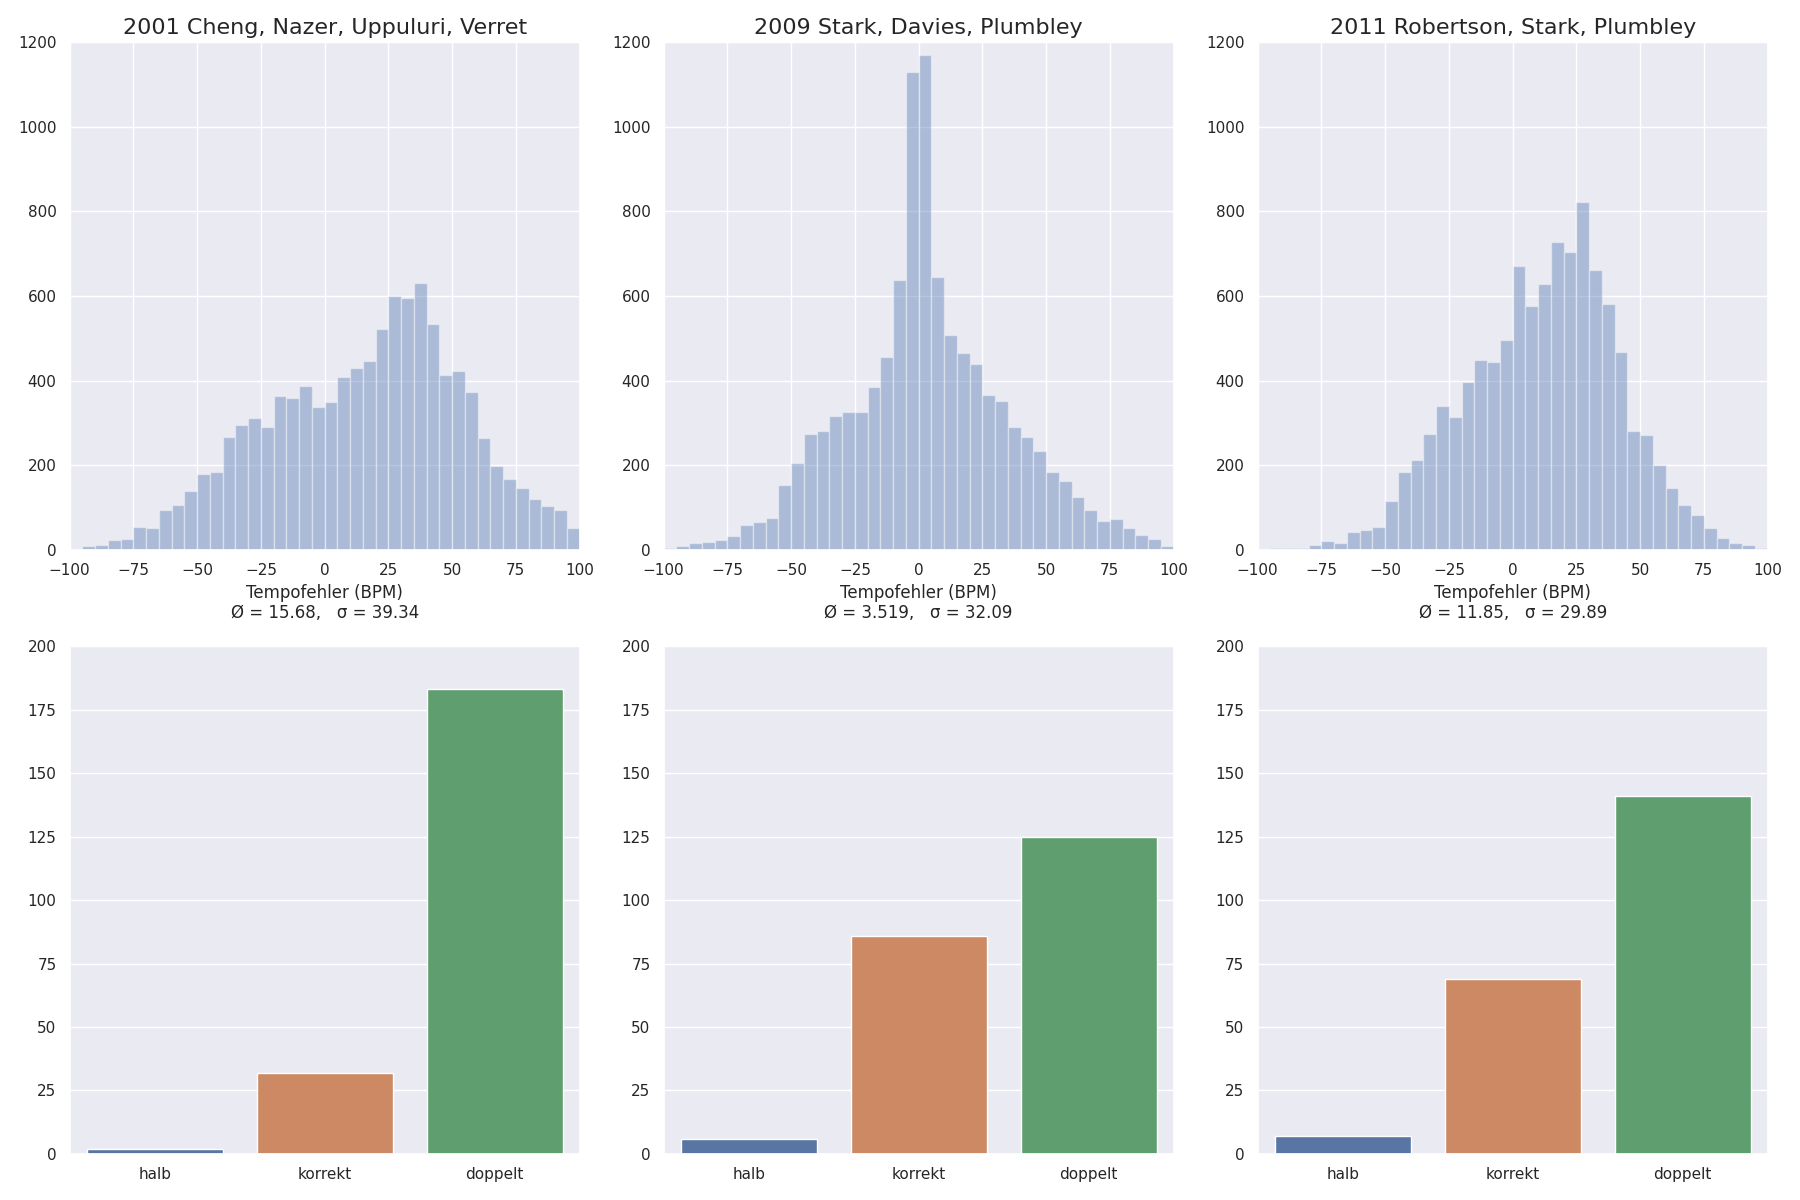
\includegraphics[scale=0.45]{resources/tempo_error_histogram.png}
			\caption{
				oben: Histogramme der Tempofehler, \\
				unten: Anzahl der Lieder, bei denen das halbe/korrekte/doppelte Tempo erkannt wurde
			}
			\label{fig:tempoerror}
		\end{figure}

		% Beschreibung Abbildung Tempofehler
		Die Histogramme in Abbildung~\ref{fig:tempoerror} zeigen die Verteilung der Tempofehler aller Lieder pro Algorithmus.
		Der abgebildete Bereich von \SIrange{-100}{100}{BPM} ist in \num{40} Balken unterteilt.
		So umfasst jeder Balken eine Spanne von \SI{5}{BPM}.
		Die Balkendiagramme zeigen pro Algorithmus,
			bei wievielen Liedern das halbe, das korrekte oder das doppelte Tempo als Referenztempo genommen wurde.

		% Auffälligkeiten der Abblidung
		Man kann deutlich erkennen,
			dass die Algorithmen von~\cite{2001_BeatThis} und~\cite{2011_PlRoSt} im Durchschnitt das Tempo etwas zu schnell schätzen.
		\cite{2009_DaPlSt} hingegen weicht im Durchschnitt nur minimal von einem Fehler von 0 ab und
			hat mehr Fehler, die sehr nah an 0 sind.
		Am meisten gestreut sind die Fehler bei \cite{2001_BeatThis}.
		Die Fehler von~\cite{2009_DaPlSt} haben zwar eine etwas größere Streuung (Standardabweichung) als die von~\cite{2011_PlRoSt},
			trotzdem kann man aber sagen,
			dass~\cite{2009_DaPlSt} in diesem Vergleich die besten Tempovorhersagen macht,
			da der Durchschnittsfehler viel näher an 0 ist.

		\begin{figure}[h]
			\centering
			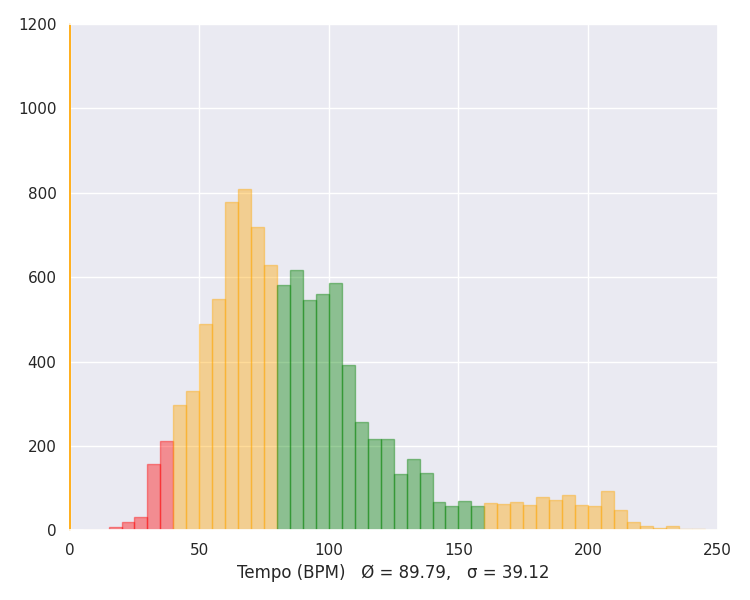
\includegraphics[scale=0.45]{resources/dataset_tempo_histogram.png}
			\caption{Tempoverteilung des Datensatzes}
			\label{fig:dataset_tempo}
		\end{figure}

		Auffällig ist außerdem,
			dass bei jedem Algorithmus die meisten Lieder mit dem doppelten Tempo erkannt wurden.
		Das ist hauptsächlich dem limitierten Ausgabebereich der Algorithmen von \SIrange{80}{160}{BPM} zu verschulden.
		Abbildung~\ref{fig:dataset_tempo} zeigt die Verteilung der Tempi aller Beatintervalle im Datensatz.
		Der grüne Bereich enthält \SI{44.44}{\percent} aller Beatintervalle
			und markiert den Tempobereich,
			den die Algorithmen direkt ausgeben können (\SIrange{80}{160}{BPM}).
		Der gelbe Bereich markiert den Tempobereich,
			den die Algorithmen mit Berücksichtigung von Halb- und Doppeltempofehler ausgeben können,
			also von \SIrange{40}{80}{BPM} und von \SIrange{160}{320}{BPM},
			und enthält \SI{51.45}{\percent} aller Beatintervalle,
			wobei sich die meisten davon im untern Tempoberiech befinden.
		Das erklärt,
			warum so viele Lieder mit doppeltem Tempo erkannt wurden.
		Der rote Berech ist alles was außerhalb von \SIrange{40}{320}{BPM} ist
			und markiert den Tempobereich,
			den die Algorithmen unmöglich bestimmen können.
		Dieser Bereich enthält \SI{4.11}{\percent} aller Beatintervalle.
	}

	\subsection{Auswertung}
	{

		% Mögliche Erklärung 1 (ODF)
		Eine mögliche Erklärung,
			warum~\cite{2001_BeatThis} ungenauere Tempovorhersagen macht,
			ist,
			dass der Algorithmus eine einfachere Einsatzdetektionsfunktion (ODF von engl. onset detection function) verwendet.
		Die ODF basiert auf einer Glättung und einer anschliesenden Differentiation.
		So werden nur schnelle Anstiege der Lautstärke extrahiert,
			während bei der ODF der anderen beiden Algorithmen auch die Änderungen der Phase im Signal berücksichtigt werden
			und so auch Tonänderungen,
			bei denen die Lautstärke gleich bleibt,
			als Einsätze erkannt werden.

		% Mögliche Erklärung 2 (Tempo Induction)
		Außerdem verwendet~\cite{2001_BeatThis} zur Tempobestimmung Kammfilter mit drei Zähnen,
			welche einen ähnlichen Effekt wie eine Autokorrelationsfunktion (ACF von engl. auto correlation function) haben.
		Bei der ACF wird das Signal mit einer verzögerten Version von sich selbst elementweise multipliziert.
		Bei diesem Kammfilter wird das Signal mit zwei verzögerten Versionen von sich selbst elementweise addiert.
		Beide Operationen haben den Effekt,
			dass sich,
			bei der richtigen Verzögerung,
			die regelmäsigen Peaks des Signals überlagern
			und so die Ausgabe einen großen Wert annimmt.
		Weil ein Signal,
			was sich beispielsweise alle $T$ Sekunden wiederholt,
			sich gleichzeitig auch alle $2T, 3T,$ usw. Sekunden wiederholt,
			entstehen in der ACF sowie in der Kammfilterausgabe mehrere Peaks jeweils bei Vielfachen des ersten Peaks.
		\cite{2001_BeatThis} hört an dieser Stelle auf
			und bestimmt einfach den größten Peak als Beatperiode des Songs,
			während die anderen Peaks ignoriert werden.
		\cite{2009_DaPlSt} hingegen multipliziert anschließend die Ausgabe der ACF mit mehreren Kammfiltern
			um die Abstände von äquidistanten Peaks in der ACF zu ermitteln.

		% 2009 vs. 2011 (vorverarbeitete ODF)
		Die Tempobestimmung von~\cite{2011_PlRoSt} lässt sich schwierig mit der der anderen beiden Algorithmen vergleichen,
			da sie auf einem komplett anderen Prinzip aufbaut.
		Es lässt sich aber in der Visualisierung der Algorithmen erkennen,
			dass die vorverarbeitete ODF von~\cite{2009_DaPlSt} deutlichere und prägnantere Peaks hat,
			als die von~\cite{2011_PlRoSt}.
		Das könnte teilweise die unterschiedlichen Ergebnisse dieser beiden Algorithmen erklären.

		% 2009 vs. 2011 (Einlaufzeit)
		Eine weitere Erklärung für die schlechteren Ergbnisse von~\cite{2011_PlRoSt} könnte eine längere Einlaufzeit sein.
		Vielleicht ist die Tempovorhersage am Ende des Songs nicht ungenauer als die von~\cite{2009_DaPlSt}
			und der Algorithmus braucht nur länger um darauf zu kommen,
			weshalb am Anfang des Songs viele Tempovorhersagen falsch seien könnten
	}
}

\section{Beatzeitpunktfehler}
{
	\begin{figure}[h]
		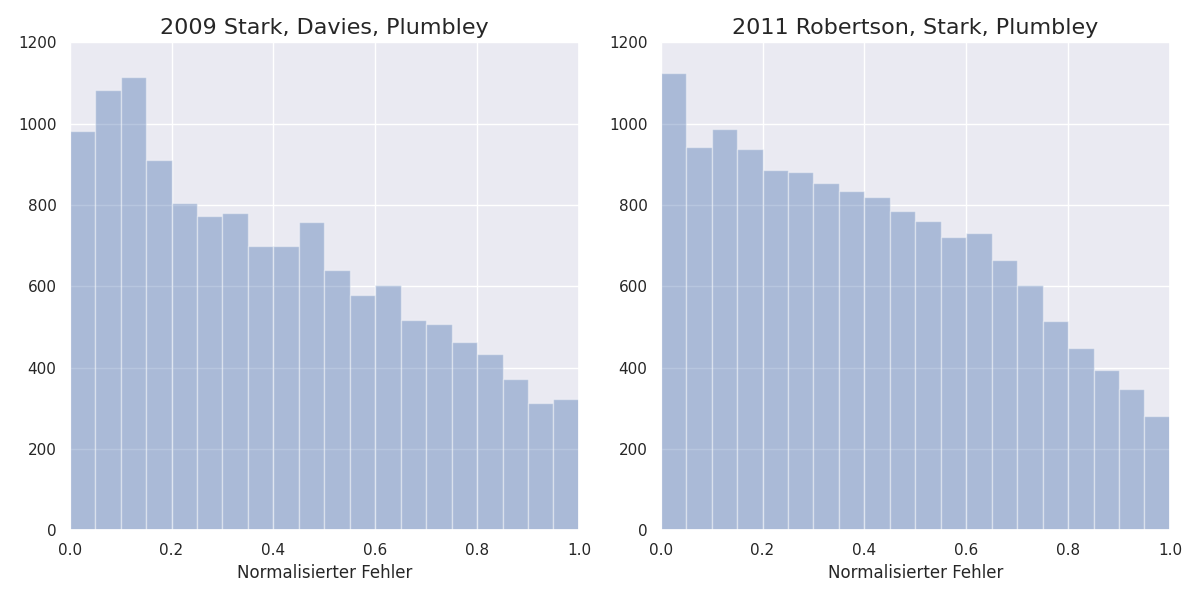
\includegraphics[scale=0.5]{resources/beat_positions.png}
		\caption{
			oben: Histogramme der Beatzeitpunktfehler, \\
			mitte: Verteilung der längsten korrekten Beatfolgen, \\
			unten: Anzahl der Lieder, bei denen die Beatfolge mit halbem/korrektem/doppeltem Tempo erkannt wurde.
		}
		\label{fig:beaterror}
	\end{figure}

	In Abbildung~\ref{fig:beaterror} oben ist die Verteilung der Fehler aller Beatpaare zu sehen,
		inklusive der Fehler der ungepaarten Schläge,
		welche immer \num{1} sind.
	Die Graphen in der Mitte zeigen eine vertikel gespiegelte kumulative Verteilunsfunktion.
	So kann man für jede Beatfolgenlänge ablsesen,
		in wievielen Liedern (prozentual) eine korrekte Beatfolge mit mindestens dieser Länge erkannt wurde.
	Die Balkendiagramme zeigen pro Algorithmus,
		bei wievielen Liedern eine Beatfolge mit halbem, korrektem oder doppeltem Tempo als Referenzbeatfolge genommen wurde.
	Ob die Referenzbeatfolge um $\pi$ phasenverschoben wurde, oder nicht, ist nicht zu sehen.
}

\section{längste korrekte Beatfolge}
{
	Die längste korrekte Beatfolge von~\cite{2009_DaPlSt} ist \num{86}.
	\cite{2011_RoPlSt} hingegen hat Beatfolge von \num{39} Schlägen korrekt erfasst.
}

\section{Rechenzeit}
{
}
